\documentclass[11pt,a4paper]{article}
\usepackage[utf8]{inputenc}
%\usepackage[T1]{fontenc}
\usepackage{graphicx}
\usepackage{longtable}
\usepackage{float}
\usepackage{wrapfig}
\usepackage{rotating}
\usepackage[normalem]{ulem}
\usepackage{amsmath}
\usepackage{textcomp}
\usepackage{marvosym}
\usepackage{wasysym}
\usepackage{amssymb}
\usepackage{hyperref}
\usepackage{listings}
\usepackage{verbatim}
\tolerance=1000
\bibliographystyle{plain}
\usepackage{microtype}
\usepackage{tikz}
\usepackage{circuitikz}
\usetikzlibrary{tikzmark,decorations.pathmorphing}
\author{Sasja Gillissen, Martin Huijben, Martijn Terpstra}
\date{\today}
\title{Testing Techniques\\
  \textbf{Assignment 2}}
\hypersetup{
 pdfauthor={Sasja Gillissen, Martin Huijben, Martijn Terpstra},
 pdflang={English}}
\begin{document}
\maketitle
%\tableofcontents

%% The purpose of this assignment is to apply automated testing and
%% Model-Based Testing (MBT) to your System Under Test (SUT). The
%% first step will be to automatically execute the manual test cases
%% that you developed in the first assignment. In the second step you
%% will apply the MBT tool TorXakis. Try to combine both parts as much
%% as possible, i.e., automate your test-execution in part 1 in such a
%% way, that you can reuse large parts of it for MBT in part 2.

\section{Automated Test Execution}
%% Automate the execution of your manually developed test cases:

In our previous assignment we developed the following use cases

\begin{center}
\begin{tabular}{llr}
Category & Input & Expected Output\\
\hline
Exiting & \texttt{exit} & Nothing\\
Function Assignment & \texttt{f(x):= x + 1 ; f(7)} & \texttt{8}\\
Builtin Functions (1) & \texttt{sqrt(ln(log(100)))} & \texttt{0.83}\\
Builtin Functions (2) & \texttt{floor(0.5) + ceil(0.5) + round(0.5)} & \texttt{2}\\
Variable Assignment & \texttt{k = 3 ; k} & \texttt{3}\\
Builtin Variables & \texttt{e * pi} & \texttt{8.5397342226735656}\\
Expression (1) & \texttt{(((0 + 1) * 2) - 3) / 4} & \texttt{-0.2500000000000000}\\
Expression (2) & \texttt{1 / 0} & Error\\
Equality (1) & \texttt{3 = 3} & \texttt{0}\\
Equality (2) & \texttt{2 = 1} & \texttt{1}\\
Equality (3) & \texttt{2 = 3} & \texttt{-1}\\
\end{tabular}
\end{center}

\subsection{Describe, design, and develop an automated test execution environment for your SUT.}
%% You may use any additional (test) tools that you think are useful,
%% e.g., search the Web for test execution tools, such as Selenium,
%% JuBuLa, scripting languages, a protocol sniffer, . . .

Our SUT is deterministic so for any given input we can expect the
same output. As such we can simply test each use case by supplying
input for each test case and seeing if the output matches.

For each use case we create 3 files with the post fixes
``\_{}input.txt'' ``\_{}output.txt'' and ``\_{}errors.txt''. The first
is the input we give the SUT, the other two being the expected
outputs. These are split in two since UNIX shells output to both
STDOUT (normal output) and STDERR(errors). Some of our use cases
except the SUT to throw error output so this is included.

For the actual test we have written a simple bash script that.

\begin{itemize}
\item For each test pipes the input into our SUT and writes the output and errors to a file
\item Compares the outputs with the expected output using the ``diff'' command
\item If the outputs match simply echo ``[OK]''
\item If the outputs don't match, show a diff of the outputs outlining what was different.
\end{itemize}

The SUT passes all tests if all test cases return ``[OK][OK]''

\subsection{Implement the test cases that you developed for manual testing, as scripts, programs, text files, . . . , so that they can be executed with your test execution environment.}

The full code, including the use cases can be found at \url{https://github.com/Witik/CommandlineCalculator}
%% TODO: make code fit page

\subsection{Test your SUT with the automated test scripts and analyze the results.}

This is the final output of our test script

\begin{verbatim}
exit:                 [OK][OK]
function_assignment:  [OK][OK]
builtin_function1:    [OK][OK]
builtin_function2:    [OK][OK]
variable_assignment:  [OK][OK]
builtin_variables:    [OK][OK]
expression1:          [OK][OK]
expression2:          [OK][OK]
equality1:            [OK][OK]
equality2:            [OK][OK]
equality3:            [OK][OK]
\end{verbatim}

The result is unsurprising, each test is successful. Since we had
previously defined all use cases in detail making correct tests turned out to be easy.

\subsection{Evaluate your automated test execution environment.}

Since we had previously made very concrete test cases and our program
can be communicated with from the command line automation was easy.
Once our script could test the first use case, the remaining ten use
cases could be added to the test suite in a matter minutes.

The testing suite was kept simple, allowing to to be developed in a
lunch break. It would most likely have taken longer to look for a
tool, learn it and set it up. The full testing environment could be
setup in a fraction of the time it took us to get TorXakis working.

Furthermore because of its simplicity it was trivial to add use cases.
Which means that if our SUT would later gain more features we could
easily add more use cases to test for.


\section{Model-Based Testing}
%% Use the MBT tool TorXakis
%% (http://www.cs.ru.nl/personal/tretmans/torxakis/) to model and test
%% your SUT:

\subsection{Modeling Investigation}
We wanted to model the use cases we made in the previous assignment. Here they are again:

\begin{center}
	\begin{tabular}{llr}
		Category & Input & Expected Output\\
		\hline
		Exiting & \texttt{exit} & Nothing\\
		Function Assignment & \texttt{f(x):= x + 1 ; f(7)} & \texttt{8}\\
		Builtin Functions (1) & \texttt{sqrt(ln(log(100)))} & \texttt{0.83}\\
		Builtin Functions (2) & \texttt{floor(0.5) + ceil(0.5) + round(0.5)} & \texttt{2}\\
		Variable Assignment & \texttt{k = 3 ; k} & \texttt{3}\\
		Builtin Variables & \texttt{e * pi} & \texttt{8.5397342226735656}\\
		Expression (1) & \texttt{(((0 + 1) * 2) - 3) / 4} & \texttt{-0.2500000000000000}\\
		Expression (2) & \texttt{1 / 0} & Error\\
		Equality (1) & \texttt{3 = 3} & \texttt{0}\\
		Equality (2) & \texttt{2 = 1} & \texttt{1}\\
		Equality (3) & \texttt{2 = 3} & \texttt{-1}\\
	\end{tabular}
\end{center}


%% Investigate and study (the behaviour of) your SUT; investigate and argue which parts of your SUT, which interfaces, and which functionality might be tested with TorXakis.

\subsection{MBT Modeling}
%% Make a model for your SUT in the TorXakis modelling language txs.}
%% Explain your model (structure, processes, data definitions, . . . ).

\subsection{MBT Test Environment}
%% Develop a test environment or test architecture which will be used for model-based testing of your SUT.}
%% Give a sketch of the test architecture, i.e., the positioning of the
%% SUT, test tool(s), adapter(s), logging tool(s), . . ., and their
%% connections and interfaces; explain your choices. Try to reuse the
%% test-execution automation environment as much as possible.

Our main application, Commandlinecalculator is a command line tool

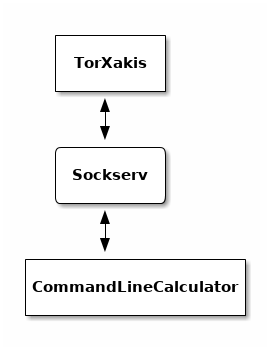
\includegraphics[width=8cm]{overview.png}

\subsection{MBT Testing}
%% Use TorXakis to generate tests, and execute them on your SUT.}
%% Explain your observations and analyse the test results.

\subsection{Deliverable}
%% Give the models, code, adapters, etc. in such a way that we can run it; provide a ’README’.}
%% Be prepared to give a demo.


\end{document}

%%  LocalWords:  tikzmark pathmorphing Sasja Gillissen Huijben MBT ln
%%  LocalWords:  pdfauthor pdflang TorXakis SUT llr sqrt ceil JuBuLa
%%  LocalWords:  txt STDOUT STDERR
